\documentclass[runningheads]{llncs}

\usepackage[T1]{fontenc}
\usepackage{graphicx}
% \renewcommand\UrlFont{\color{blue}\rmfamily}
\usepackage{hyperref}
\usepackage{color}
\usepackage{setspace}
\usepackage{verbatim}
\usepackage{multicol}
\usepackage{array}
\usepackage{bbding}
\usepackage{wasysym}

%----Making things more compact
\newcommand{\smalltt}[1]{\small \texttt{#1}}
\newenvironment{packed_itemize}{
\vspace*{-0.2em}
\begin{itemize}
\setlength{\partopsep}{0pt}
\setlength{\itemsep}{1pt}
\setlength{\parskip}{0pt}
\setlength{\parsep}{0pt}
}{\end{itemize}}
\newenvironment{packed_enumerate}{
\vspace*{-0.2em}
\begin{enumerate}
\setlength{\partopsep}{0pt}
\setlength{\itemsep}{1pt}
\setlength{\parskip}{0pt}
\setlength{\parsep}{0pt}
}{\end{enumerate}}
\renewcommand{\textfraction}{0.07}
\renewcommand{\topfraction}{0.9}
\renewcommand{\bottomfraction}{0.9}
\renewcommand{\floatpagefraction}{0.66}
\setlength{\floatsep}{2.0pt plus 2.0pt minus 2.0pt}
\setlength{\textfloatsep}{5.0pt plus 2.0pt minus 0.0pt}

\title{Automated Reasoning for Mathematics \\ in the TPTP World}

\author{
  Geoff Sutcliffe\orcidID{0000-0001-9120-3927}\Envelope
}

\institute{
  University of Miami,
  Miami, USA\\
  \email{geoff@cs.miami.edu}\\
}

\authorrunning{Geoff Sutcliffe}
\titlerunning{Mathematics in the TPTP World}

\begin{document}
\maketitle

%--------------------------------------------------------------------------------------------------
\begin{abstract}
The TPTP World is a well established infrastructure that supports research, development, and 
deployment of Automated Theorem Proving (ATP) systems.
A large portion of the TPTP is concerned with various mathematical domains.
This paper documents the mathematical domains of TPTP v9.0.0, and provides some insight into 
the performance of state-of-the-art ATP systems on the problems in these domains.
For those new to the field this information provides an established starting point for research.
For those already involved, this paper tells what has been achieved so far.
\end{abstract}
%--------------------------------------------------------------------------------------------------
\section{Introduction}
\label{Introduction}

Automated Reasoning is a subfield of artificial intelligence, dealing with computer systems
(largely software systems) that allow computers to reason completely, or nearly completely, 
automatically\footnote{%
Quoted from Wikipedia \href{https://en.wikipedia.org/wiki/Automated_reasoning}{{\tt en.wikipedia.org/wiki/Automated\_reasoning}}}~\cite{RV01-HAR}.
Automated reasoning spans a diversity of approaches, from deduction in logic~\cite{Gal15} to more 
forgiving types of reasoning such as argumentation~\cite{vE+14}.
The left side of Figure~\ref{UseOfAR} shows how automated reasoning systems are used in general: 
(i)~a world problem written in the language of the application domain is translated to the language
of the automated reasoning system; (ii)~the resultant reasoning problem is given to an automated 
reasoning system; (iii)~the automated reasoning system produces a solution (which can be in a
language different from that used for the problem); (iv)~the solution is translated to the 
language of the application domain.

For automated reasoning in mathematics, the mathematical problems are very often translated to 
a formal logic language, and the automated reasoning systems used to solve the problems are 
Automated Theorem Proving (ATP) systems~\cite{Bun83,RV01-HAR}.
The right side of Figure~\ref{UseOfAR} shows the specialization of general automated reasoning
to mathematical reasoning in logic:
(i)~a mathematical problem written in a mathematical language is translated to an appropriate 
logic language, as a set of axioms that model the mathematical domain, typically accompanied 
by a conjecture that formalizes a theorem to be proved; (ii)~the resultant logic problem is given 
to an ATP system; (iii)~the ATP system produces a solution in a logic language (which can be 
in a logic language different from that used to write the problem); (iv)~the logic solution is 
translated to a solution in a mathematical language.

\begin{figure}[htb]
\centering
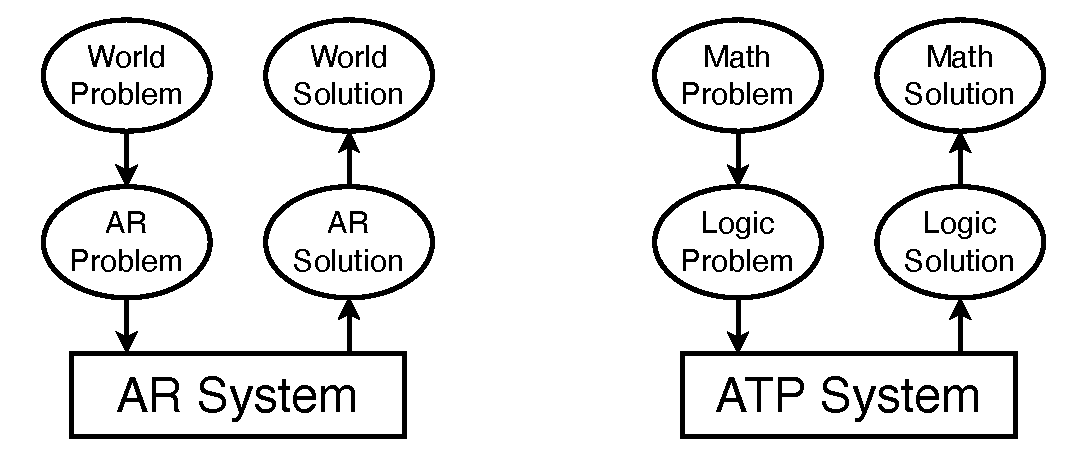
\includegraphics[width=0.6\textwidth]{UseOfAR.pdf}
\vspace*{-1em}
\caption{Use of Automated Reasoning}
\label{UseOfAR}
\end{figure}

The TPTP World is a well established infrastructure that supports research, development, and 
deployment of ATP~\cite{Sut10,Sut17}.
A large portion of the TPTP World is concerned with various mathematical domains, problems, and
solutions.
This paper describes the content and services of the TPTP World that support automated reasoning
in mathematics.
Section~\ref{TPTPWorld} provides the necessary background about the TPTP World.
Section~\ref{MathProblems} describes the breadth and depth of mathematical problems in the TPTP
World.
Section~\ref{MathSolutions} covers the solutions to mathematical problems in the TPTP World,
including some details of outstanding results in mathematics achieved with ATP.
Section~\ref{Conclusion} concludes.

%--------------------------------------------------------------------------------------------------
\section{The TPTP World}
\label{TPTPWorld}

This section describes the parts of the TPTP World that are referred to in the subsequent sections 
that describe the mathematics in the TPTP World.
Salient components of the TPTP World are
the TPTP language that is used to write mathematical problems and solutions as logic problems and 
solutions (Section~\ref{Languages}),
the TPTP problem library and TSTP solution library that contain (amoung others) mathematical
problems and solutions (Section~\ref{TPTPTSTP}),
the problem and ATP systems ratings that indicate how hard (the mathematical) problems are and 
how strong the ATP systems are (Section~\ref{Ratings}),
and SystemOnTPTP for executing ATP systems and tools on the mathematical problems and solutions
(Section~\ref{SystemOnTPTP}).
The web page \href{http://www.tptp.org}{{\tt www.tptp.org}} provides access to all components.

%--------------------------------------------------------------------------------------------------
\subsection{The TPTP Language}
\label{Languages}

The TPTP language~\cite{Sut23-IGPL} is one of the keys to the success of the TPTP World.
The TPTP language is used for writing both problems and solutions,
which enables convenient communication between ATP systems and tools.
The TPTP language supports propositional, first-order, typed first-order, higher-order, and
non-classical logics, each of which is useful for different types of mathematics.

Problems and solutions are built from {\em annotated formulae} of the form: \\
\hspace*{0.5cm}{\em language}{\tt (}{\em name}{\tt ,}
{\em role}{\tt ,}
{\em formula}{\tt ,}
{\em source}{\tt ,}
{\em useful\_info}{\tt )}\\
The {\em language}s supported are {\smalltt{cnf}} (clause normal form), {\smalltt{fof}}
(first-order form), {\smalltt{tff}} (typed first-order form), and {\smalltt{thf}}
(typed higher-order form).
The {\em role}, e.g., {\smalltt{axiom}}, {\smalltt{lemma}}, {\smalltt{conjecture}}, defines the 
use of the formula.
In a {\em formula}, terms and atoms follow Prolog conventions -- functions and predicates start 
with a lowercase letter or are {\tt '}single quoted{\tt '}, and variables start with an uppercase 
letter.
The language also supports interpreted symbols that either start with a {\tt \$}, e.g., the 
truth constants {\smalltt{\$true}} and {\smalltt{\$false}}, or are composed of 
non-alphabetic characters, e.g., integer/rational/real numbers such as 27, 43/92, -99.66.
The logical connectives in the TPTP language are
{\tt !}, {\tt ?}, {\tt {\raisebox{0.4ex}{\texttildelow}}}, {\tt |}, {\tt \&}, {\tt =>}, {\tt <=},
{\tt <=>}, and {\tt <{\raisebox{0.4ex}{\texttildelow}}>},
for the mathematical connectives
$\forall$, $\exists$, $\neg$, $\vee$, $\wedge$, $\Rightarrow$, $\Leftarrow$, $\Leftrightarrow$, 
and $\oplus$ respectively.
Equality and inequality are expressed as the infix operators {\tt =} and {\tt !=}.
The {\em source} and {\em useful\_info} are optional.
Figure~\ref{ExampleFOF} shows an example set theory problem written in first-order logic
(it is the TPTP problem {\tt SET002+3}), and Figure~\ref{ExampleTF0} shows an example
arithmetic problem written in typed first-order logic (it is the TPTP problem {\tt ARI740\_1}).

\begin{figure}[htb]
\centering
{\footnotesize
{\setlength{\baselineskip}{3mm}
\begin{verbatim}
%------------------------------------------------------------------------
fof(subset_union,axiom,
    ! [B,C] : ( subset(B,C) => union(B,C) = C ) ).

fof(union_defn,axiom,
    ! [B,C,D] :
      ( member(D,union(B,C)) <=> ( member(D,B) | member(D,C) ) ) ).

fof(equal_defn,axiom,
    ! [B,C] :
      ( B = C <=> ( subset(B,C) & subset(C,B) ) ) ).

fof(commutativity_of_union,axiom,
    ! [B,C] : union(B,C) = union(C,B) ).

fof(subset_defn,axiom,
    ! [B,C] :
      ( subset(B,C)
    <=> ! [D] : ( member(D,B) => member(D,C) ) ) ).

fof(reflexivity_of_subset,axiom,
    ! [B] : subset(B,B) ).

fof(equal_member_defn,axiom,
    ! [B,C] :
      ( B = C
    <=> ! [D] : ( member(D,B) <=> member(D,C) ) ) ).

fof(prove_idempotency_of_union,conjecture,
    ! [B] : union(B,B) = B ).
%------------------------------------------------------------------------
\end{verbatim}
}}
\caption{Set theory in first-order logic}
\label{ExampleFOF}
\end{figure}

\begin{figure}[htb]
\centering
{\footnotesize
{\setlength{\baselineskip}{3mm}
\begin{verbatim}
%------------------------------------------------------------------------
tff(power,type, power: ( $real * $int ) > $real ).

tff(power_0,axiom,
    ! [X: $real] : ( power(X,0) = 1.0 ) ).

tff(power_s,axiom,
    ! [X: $real,N: $int] :
      ( $lesseq(0,N) 
     => ( power(X,$sum(N,1)) = $product(X,power(X,N)) ) ) ).

tff(power_s_alt,axiom,
    ! [X: $real,N: $int] :
      ( $less(0,N) 
     => ( power(X,N) = $product(X,power(X,$difference(N,1))) ) ) ).

tff(power_1,axiom,
    ! [X: $real] : ( power(X,1) = X ) ).

tff(power_sum,axiom,
    ! [X: $real,N: $int,M: $int] :
      ( $lesseq(0,N)
     => ( $lesseq(0,M) 
       => ( power(X,$sum(N,M)) = $product(power(X,N),power(X,M)) ) ) ) ).

tff(power_mult,axiom,
    ! [X: $real,N: $int,M: $int] :
      ( $lesseq(0,N)
     => ( $lesseq(0,M) 
       => ( power(X,$product(N,M)) = power(power(X,N),M) ) ) ) ).

tff(power_mult2,axiom,
    ! [X: $real,Y: $real,N: $int] :
      ( $lesseq(0,N)
     => ( power($product(X,Y),N) = $product(power(X,N),power(Y,N)) ) ) ).

tff(pow_ge_one,axiom,
    ! [X: $real,N: $int] :
      ( ( $lesseq(0,N) & $lesseq(1.0,X) ) => $lesseq(1.0,power(X,N)) ) ).

tff(pow_2_2,conjecture,
    power(2.0,2) = 4.0 ).
%------------------------------------------------------------------------
\end{verbatim}
}}
\caption{Arithmetic in typed first-order logic}
\label{ExampleTF0}
\end{figure}

%--------------------------------------------------------------------------------------------------
\subsection{The TPTP Problem and Solution Libraries}
\label{TPTPTSTP}

The TPTP problem library is a comprehensive library of test problems for ATP systems~\cite{Sut09}.
It supports necessary for meaningful ATP system evaluations, meaningful system comparisons, 
repeatability of testing, and the production of statistically significant results. 
The problems are classified into {\em domains} that reflect a natural hierarchy,
based mainly on the Dewey Decimal Classification and the Mathematics Subject Classification.
Seven main fields are defined: logic, mathematics, computer science, science \& engineering, 
social sciences, arts \& humanities, and other. 
Each field is subdivided into domains, each identified by a three-letter mnemonic.
For a given {\em abstract} mathematical problem the TPTP problem library can have multiple 
concrete {\em versions}, which are the problems that ATP systems solve. 

Each problem version is stored in a separate physical file, using the naming scheme {\em DDDNNNFV}.
{\em DDD} is the domain mnemonic, {\em NNN} is the index of the abstract problem in the domain,
{\em F} identifies the TPTP language, and {\em V} is the version index in the abstract problem.
Each problem file has three parts: a header, optional includes, and annotated formulae.
The header section contains information for users, formatted as comments in four parts, as shown
in Figure~\ref{ExampleHeader}.
The first part identifies and describes the problem,
the second part provides information about occurrences of the problem
in the literature and elsewhere,
the third part provides semantic and syntactic characteristics of the problem, and
the last part contains comments and bugfix information.
The header fields are self-explanatory, but of particular interest are the {\tt Status} field 
that is explained in Section~\ref{SZS}, the {\tt Rating} field that is explained in 
Section~\ref{Ratings}, and the {\tt SPC} field that is explained in Section~\ref{SPCs}.
The include section is optional, and if used contains {\tt include} directives for axiom files,
which in turn have the same three-part format as problem files; see Figure~\ref{ExampleHeader}
for an example.
Inclusion avoids the need for duplication of the formulae in commonly used axiomatizations.
The annotated formulae are described in Section~\ref{Languages}, and Figure~\ref{ExampleFormulae} 
provides an example.

\begin{figure}[htb]
\centering
{\scriptsize
{\setlength{\baselineskip}{2.5mm}
\begin{verbatim}
%------------------------------------------------------------------------------
% File     : DAT016_1 : TPTP v8.2.0. Bugfixed v5.1.0.
% Domain   : Data Structures
% Problem  : Some element is 53
% Version  : [PW06] axioms.
% English  : Show that some element of the array has the value 53.

% Refs     : [PW06]  Prevosto & Waldmann (2006), SPASS+T
%          : [Wal10] Waldmann (2010), Email to Geoff Sutcliffe
% Source   : [Wal10]
% Names    : (40) [PW06]

% Status   : Theorem
% Rating   : 0.25 v8.2.0, 0.12 v7.5.0, 0.30 v7.4.0, 0.12 v7.3.0, etc.
% Syntax   : Number of formulae    :    6 (   1 unt;   3 typ;   0 def)
%            Number of atoms       :   12 (   5 equ)
%            Maximal formula atoms :    4 (   2 avg)
%            Number of connectives :    4 (   0   ~;   1   |;   1   &)
%                                         (   0 <=>;   2  =>;   0  <=;   0 <~>)
%            Maximal formula depth :    6 (   5 avg)
%            Maximal term depth    :    3 (   1 avg)
%            Number of FOOLs       :    5 (   5 fml;   0 var)
%            Number arithmetic     :   16 (   2 atm;   2 fun;   5 num;   7 var)
%            Number of types       :    2 (   1 usr;   1 ari)
%            Number of type conns  :    5 (   2   >;   3   *;   0   +;   0  <<)
%            Number of predicates  :    3 (   1 usr;   0 prp; 2-2 aty)
%            Number of functors    :    9 (   2 usr;   5 con; 0-3 aty)
%            Number of variables   :   10 (   9   !;   1   ?;  10   :)
% SPC      : TF0_THM_EQU_ARI

% Comments : The array contains integers.
% Bugfixes : v5.1.0 - Fixed conjecture
%------------------------------------------------------------------------------
%----Includes axioms for arrays
include('Axioms/DAT001_0.ax').
%------------------------------------------------------------------------------
\end{verbatim}
}}
\caption{Header of problem {\tt DAT016\_1}.}
\label{ExampleHeader}
\end{figure}

The complement to the TPTP problem library is the TSTP solution library~\cite{Sut07-CSR,Sut10}.
The TSTP is built by running all the ATP systems that are available in the TPTP World on
all the problems in the TPTP problem library.
The TSTP started being built around 2005, using solutions provided by individual system developers.
From 2010 to 2013 the TSTP was generated on a small NSF funded\footnote{%
NSF Award 0957438} cluster at the University of Miami.
Since 2014 the ATP systems have been run on StarExec (see Section~\ref{StarExec}), initially on 
the StarExec Iowa cluster, and since 2018 on the StarExec Miami cluster.
StarExec has provided stable platforms that produce reliably consistent and comparable data in 
the TSTP.
% The ATP systems come from a range of sources:
% some were developed many years ago and are no longer distributed;
% some are the most recent available, taken either from the systems’ web sites or from the most 
% recent edition of CASC.
At the time of writing this paper the TSTP contained the results of running 87 ATP systems and 
system variants on all the problems that each system could attempt
(therefore, e.g., systems that do model finding for FOF are not run on THF problems).
This produced 1091026 runs, of which 432718 (39.6\%) solved the problem.
One use of the TSTP is for computing the TPTP problem difficulty ratings (see 
Section~\ref{Ratings}).

TSTP solution files have a header section and annotated formulae.
The header section has four parts, as shown in Figure~\ref{ExampleDerivationHeader}:
the first part identifies the ATP system, the problem, and the system's runtime parameters; 
the second part provides information about the hardware, operating system, and resource limits; 
the third part provides the SZS result and output values (see Section~\ref{SZS}), and syntactic 
characteristics of the solution; the last part contains comments.
The solution follows in annotated formulae.

For derivations, where formulae are derived from parent formulae, e.g., in proofs, refutations, 
etc., the {\em source} fields of the annotated formulae are used to capture parent-derived 
formulae relationships in the derivation DAG.
This includes the source of the formula -- either the problem file or an inference.
Inference data includes the name of the inference rule used, the semantic relationship between 
the parents and the derived formula as an SZS ontology value (see Section~\ref{SZS}), and a 
list of the parent annotated formulae names.
Figure~\ref{ExampleDerivationFormulae} shows an example refutation [slightly modified, type
declarations omitted] from the E system~\cite{SCV19} for the problem formulae in 
Figure~\ref{ExampleFormulae}, and Figure~\ref{ExampleDerivationHeader} shows the corresponding 
header fields.

\begin{figure}[htb]
\centering
{\scriptsize
{\setlength{\baselineskip}{2.5mm}
\begin{verbatim}
%------------------------------------------------------------------------------
% File     : E---3.0.04
% Problem  : Coffee 
% Transfm  : none
% Format   : tptp:raw
% Command  : run_E %s %d THM

% Computer : quokka.cs.miami.edu
% Model    : x86_64 x86_64
% CPU      : Intel(R) Xeon(R) CPU E5-2609 v2 @ 2.50GHz
% Memory   : 64222MB
% OS       : Linux 3.10.0-1160.36.2.el7.x86_64
% CPULimit : 30s
% WCLimit  : 0s
% DateTime : Tue Feb 13 13:29:34 EST 2024

% Result   : Theorem 0.00s 0.08s
% Output   : Refutation 0.00s
% Verified :
% SZS Type : Refutation
%            Derivation depth      :    5
%            Number of leaves      :   10
% Syntax   : Number of formulae    :   19 (   8 unt;   7 typ;   0 def)
%            Number of atoms       :   16 (   7 equ;   0 cnn)
%            Maximal formula atoms :    2 (   1 avg)
%            Number of connectives :   42 (   6   ~;   2   |;   2   &;  32   @)
%                                         (   0 <=>;   0  =>;   0  <=;   0 <~>)
%            Maximal formula depth :    7 (   5 avg)
%            Number of types       :    3 (   2 usr)
%            Number of type conns  :   11 (  11   >;   0   *;   0   +;   0  <<)
%            Number of symbols     :    7 (   5 usr;   2 con; 0-2 aty)
%            Number of variables   :   15 (   0   ^  13   !;   2   ?;  15   :)

% Comments :
%------------------------------------------------------------------------------
\end{verbatim}
}}
\caption{Example derivation header}
\label{ExampleDerivationHeader}
\end{figure}

% thf(beverage_decl,type,   beverage: $tType ).
% thf(syrup_decl,type,      syrup: $tType ).
% thf(coffee_type,type,     coffee: beverage ).
% thf(mix_type,type,        mix: beverage > syrup > beverage ).
% thf(heat_type,type,       heat: beverage > beverage ).
% thf(heated_mix_type,type, heated_mix: beverage > syrup > beverage ).
% thf(hot_type,type,        hot: beverage > $o ).
% thf(decl_27,type,         esk1_1: ( syrup > beverage ) > syrup ).
% thf(decl_28,type,         esk2_1: ( syrup > beverage ) > syrup ).

\begin{figure}[h!]
\centering
{\footnotesize
{\setlength{\baselineskip}{3mm}
\begin{verbatim}
%------------------------------------------------------------------------
thf(hot_coffee,conjecture,
    ? [X3: syrup > beverage] :
    ! [X2: syrup] :
      ( ( ( X3 @ X2 ) = coffee ) & ( hot @ ( X3 @ X2 ) ) ),
    file('Coffee.p',hot_coffee) ).

thf(heated_coffee_mix,axiom,
    ! [X2: syrup] :
      ( ( heated_mix @ coffee @ X2 ) = coffee ),
    file('Coffee.p',heated_coffee_mix) ).

thf(hot_mixture,axiom,
    ! [X1: beverage,X2: syrup] : ( hot @ ( heated_mix @ X1 @ X2 ) ),
    file('Coffee.p',hot_mixture) ).

thf(c_0_3,negated_conjecture,
    ~ ? [X3: syrup > beverage] :
      ! [X2: syrup] :
        ( ( ( X3 @ X2 ) = coffee ) & ( hot @ ( X3 @ X2 ) ) ),
    inference(assume_negation,[status(cth)],[hot_coffee]) ).

thf(c_0_4,negated_conjecture,
    ! [X16: syrup > beverage] :
      ( ( ( X16 @ ( esk1_1 @ X16 ) ) != coffee )
      | ~ ( hot @ ( X16 @ ( esk2_1 @ X16 ) ) ) ),
    inference(fof_nnf,[status(thm)],[inference(skolemize,[status(esa)],
[inference(variable_rename,[status(thm)],[inference(shift_quantors,
[status(thm)],[inference(fof_nnf,[status(thm)],[c_0_3])])])])]) ).

thf(c_0_10,negated_conjecture,
    ~ ( hot @ coffee ),
    inference(cn,[status(thm)],[inference(rw,[status(thm)],
[inference(spm,[status(thm)],[c_0_4,heated_coffee_mix]),
heated_coffee_mix])]) ).

thf(c_0_11,plain,
    $false,
    inference(sr,[status(thm)],[inference(spm,[status(thm)],
[hot_mixture,heated_coffee_mix]),c_0_10]),[proof] ).
%------------------------------------------------------------------------
\end{verbatim}
}}
\caption{Example derivation formulae}
\label{ExampleDerivationFormulae}
\end{figure}

For interpretations (typically models) the annotated formulae are used to describe the domains
and symbol mappings of Tarskian interpretations, or the formulae that induce Herbrand models.
A TPTP format for interpretations with finite domains was previously defined~\cite{SS+06}, 
and has served the ATP community adequately for almost 20 years. 
Recently the need to represent interpretations with infinite domains, and Kripke interpretations, 
has led to the development of a new TPTP format that supports these interpretations~\cite{SSP24}.
Figure~\ref{ExampleModel} shows the problem formulae and a model that uses integers as the domain.
Please read~\cite{SSP24} for lots more details!

\begin{figure}[h!]
\centering
{\footnotesize
{\setlength{\baselineskip}{3mm}
\begin{verbatim}
%---- Problem formulae --------------------------------------------------
tff(person_type,type,        person: $tType ).
tff(bob_decl,type,           bob: person ).
tff(child_of_decl,type,      child_of: person > person ).
tff(is_descendant_decl,type, is_descendant: (person * person) > $o ).

tff(descendents_different,axiom,
    ! [A: person,D: person] : 
      ( is_descendant(A,D) => ( A != D ) ) ).

tff(descendent_transitive,axiom,
    ! [A: person,C: person,G: person] :
      ( ( is_descendant(A,C) & is_descendant(C,G) ) 
     => is_descendant(A,G) ) ).

tff(child_is_descendant,axiom,
    ! [P: person] : is_descendant(P,child_of(P)) ).

tff(all_have_child,axiom,
    ! [P: person] : ? [C: person] : C = child_of(P) ).
%------------------------------------------------------------------------

%---- Model -------------------------------------------------------------
tff(person_type,type,        person: $tType ).
tff(bob_decl,type,           bob: person ).
tff(child_of_decl,type,      child_of: person > person ).
tff(is_descendant_decl,type, is_descendant: ( person * person ) > $o ).

tff(int2person_decl,type,    int2person: $int > person ).

tff(people,interpretation,
%----Domain for type person is the integers
    ( ( ! [P: person] : ? [I: $int] : int2person(I) = P
%----The type promoter is a bijection (injective and surjective)
      & ! [I1: $int,I2: $int] : 
          ( int2person(I1) = int2person(I2) => I1 = I2 ) )
%----Mapping people to integers. Note that Bob's ancestors will be 
%----interpreted as negative integers.
    & ( bob = int2person(0)
      & ! [I: $int] : child_of(int2person(I)) = int2person($sum(I,1)) )
%----Interpretation of descendancy
    & ! [A: $int,D: $int] : 
        ( is_descendant(int2person(A),int2person(D)) <=> $less(A,D) )) ).
%------------------------------------------------------------------------
\end{verbatim}
}}
\caption{Example infinite model}
\label{ExampleModel}
\end{figure}

\paragraph{Resource Limits:}
A common question, often based on mistaken beliefs, is whether the resource limits used should 
be increased to find more solutions.
Analysis shows that increasing resource limits does not significantly affect which problems 
are solved by an ATP system. 
Figure~\ref{PPPPlot} illustrates this point; it plots the CPU times taken by several contemporary 
ATP systems to solve the TPTP problems for the {\tt FOF\_THM\_RFO\_*} SPCs, in increasing order 
of time taken. 
The data was taken from the TSTP, i.e., using the StarExec Miami computers.
The relevant feature of these plots is that each system has a point at which the time taken to 
find solutions starts to increase dramatically. 
This point is called the system's Peter Principle~\cite{PH69} Point (PPP) -- it is the point at 
which the system has reached its level of incompetence. 
Evidently a linear increase in the computational resources beyond the PPP would not lead to the 
solution of significantly more problems. 
The PPP thus defines a realistic computational resource limit for the system, and if enough CPU 
time is allowed for an ATP system to reach its PPP, a usefully accurate measure of what problems 
it can solve is achieved.
% From an ATP perspective, the PPP is the point at which the ATP system gets lost in its quickly 
% growing search space. 
% Even though there may be enough memory to represent the search space at the PPP, the system is 
% largely unable to find a solution within the space. 
% The point thus also defines a realistic memory resource limit. 
The performance data in the TSTP is produced with adequate resource limits.

%--------------------------------------------------------------------------------------------------
\subsection{Problem and System Ratings}
\label{Ratings}

The TPTP problem library is divided into Specialist Problem Classes (SPCs) -- classes of problems 
with the same recognizable logical, language, and syntactic characteristics that make the
problems in each SPC homogeneous wrt ATP systems.
% SPCs added in v4.1.0 15/06/10
Evaluation of ATP systems within SPCs makes it possible to say which systems work well for what 
types of problems. 
The appropriate level of subdivision for SPCs is that at which less subdivision would merge 
SPCs for which ATP systems have distinguishable behaviour, and at which further subdivision
would unnecessarily split SPCs for which ATP systems have reasonably homogeneous behaviour.
Empirically, homogeneity is ensured by examining the patterns of system performance across the 
problems in each SPC. 
The SPCs for essentially propositional problems were motivated by the observation that 
SPASS~\cite{WA+99} performed differently on the ALC problems in the SYN domain of the TPTP.
A data-driven test for homogeneity is also possible~\cite{FS02}.

The characteristics currently used to define the SPCs in the TPTP are shown in 
Figure~\ref{SPCCharacteristics}.
Using these characteristics 223 SPCs are defined in TPTP v8.2.0. 
For example, the SPC
% Some examples are:
% {\tt CNF\_SAT\_EPR\_PEQ\_UEQ} -- clause normal form satisfiable clauses that are effectively
% propositional, have purely equality literals in unit equality clauses;
% {\tt FOF\_THM\_RFO\_SEQ} -- first-order theorems that are ``really first-order'' (not known
% to be effectively propositional), and contain some (not only) equality;
{\tt TF0\_THM\_NEQ\_ARI} contains typed monomorphic first-order theorems that have no equality but 
include arithmetic.
The header section of each problem in the TPTP problem library (see Section~\ref{TPTP}) includes 
its SPC.
The SPCs are used when computing the TPTP problems difficulty ratings (see Section~\ref{Ratings}).

\begin{figure}[bht]
\centering
\begin{packed_itemize}
\item TPTP language: \\
      \begin{tabular}{@{}p{5cm}l}
      {\tt CNF} -- Clause Normal Form &
      {\tt FOF} -- First-Order Form \\
      {\tt TF0/1} -- Typed First-order & Monomorphic/Polymorphic \\
      {\tt TX0/1} -- Typed eXtended f-o & Monomorphic/Polymorphic \\
      {\tt TH0/1} -- Typed Higher-order & Monomorphic/Polymorphic \\
      {\tt NX0/1} -- Non-classical {\tt TX0/1} &
      {\tt NH0/1} -- Non-classical {\tt TH0/1} \\
      \end{tabular}
\item SZS status: \\
      \begin{tabular}{@{}p{5cm}l}
      {\tt THM} -- Theorem &
      {\tt CSA} -- CounterSAtisfiable \\
      {\tt CAX} -- Contradictory AXioms & \\
      {\tt UNS} -- UNSatisfiable &
      {\tt SAT} -- SATisfiable \\
      {\tt UNK} -- UNKown &
      {\tt OPN} -- OPeN \\
      \end{tabular}
\item Order (for {\tt CNF} and {\tt FOF}): \\
      {\tt PRP} -- PRoPositional \\
      {\tt EPR} -- Effectively PRopositional (known to be reducible to {\tt PRP}) \\
      {\tt RFO} -- Real First-Order (not known to be reducible to {\tt PRP})
\item Equality: \\
      \begin{tabular}{@{}p{5cm}l}
      {\tt NEQ} -- No EQuality &
      {\tt EQU} -- EQUality (some or pure) \\
      {\tt SEQ} -- Some (not pure) EQuality &
      {\tt PEQ} -- Pure EQuality \\
      {\tt UEQ} -- Unit EQuality {\tt CNF} &
      {\tt NUE} -- Non-Unit Equality {\tt CNF} \\
      \end{tabular}
\item Hornness (for {\tt CNF}): \\
      \begin{tabular}{@{}p{5cm}l}
      {\tt HRN} -- HoRN &
      {\tt NHN} -- Non-HorN
      \end{tabular}
\item Arithmetic (for {\tt T*} languages): \\
      \begin{tabular}{@{}p{5cm}l}
      {\tt ARI} -- ARIthmetic &
      {\tt NAR} -- No ARithmetic
      \end{tabular}
\end{packed_itemize}
\caption{SPC characteristics}
\label{SPCCharacteristics}
\end{figure} 

Each TPTP problem has a difficulty rating that provides a well-defined measure of how difficult 
the problem is for current ATP systems~\cite{SS01}.
The ratings are based on performance data in the TSTP solution library (see Section~\ref{TSTP}), 
and are updated in each TPTP edition.

The TPTP tags problems that are designed specifically to be suited or ill-suited to some ATP
system, calculus, or control strategy as {\em biased}
(this includes the {\tt SYN000} problems, which are designed for testing ATP systems' parsers).
The biased problems are excluded from the calculations.
Rating is then done separately for each SPC (see Section~\ref{SPCs}).

First, a partial order between systems is determined according to whether or not a system 
solves a strict superset of the problems solved by another system. 
If a strict superset is solved, the first system is said to {\em subsume} the second. 
The union of the problems solved by the non-subsumed systems defines the state-of-the-art -- all 
the problems that are solved by any system. 
The fraction of non-subsumed systems that fail on a problem is the difficulty rating 
for the problem:
problems that are solved by all of the non-subsumed systems get a rating of 0.00 (easy);
problems that are solved by some of the non-subsumed systems get a rating between 0.00 and 1.00 
(difficult); 
problems that are solved by none of the non-subsumed systems get a rating of 1.00 (unsolved).
As additional output, the systems are given a rating for each SPC -- the fraction of difficult 
problems they can solve.

The TPTP difficulty ratings provide a way to assess progress in the field -- as problems that 
are unchanged are not actually getting easier, decreases in their difficulty ratings are evidence 
of progress in ATP systems.
Figures~\ref{Ratings_v5.0.0_v6.4.0} and~\ref{Ratings_v6.3.0_v8.2.0} plot the average difficulty
ratings overall and for each of the four language forms in the TPTP World (after some sensible
data cleaning).
Figure~\ref{Ratings_v5.0.0_v6.4.0} is taken from~\cite{Sut17}, published in 2017.
It plots the average ratings for the 14527 problems that had been unchanged and whose ratings 
had not been stuck at 0.00 or 1.00, from TPTP v5.0.0 that was released in 2010 to v6.4.0 that was
released in 2016. 
Figure~\ref{Ratings_v6.3.0_v8.2.0} is taken from~\cite{SK+24}, published in 2024.
It plots the average ratings for the 16236 problems that had been unchanged and whose ratings 
had not been stuck at 0.00 or 1.00, from TPTP v6.3.0 that was released in 2016 to v8.2.0 that was
released in 2023. 
The two figures’ plots dovetail quite well, which gives confidence that they really are 
comparable (there are some minor differences caused by slightly different data cleaning 
and by recent refinements to the difficulty rating calculations). 
The older plots show a quite clear downward trend both overall and for the four language forms, 
while the new plots do not. 
Possible reasons are discussed in~\cite{SK+24}.

% \begin{figure}[t!]
% \centering
% \begin{minipage}[t]{.49\textwidth}
%   \centering
%   \includegraphics[width=\textwidth]{RatingsDecline_v5.0.0_v6.4.0.pdf}
%   \vspace*{-2em}
%   \caption{Ratings from v5.0.0 to v6.4.0}
%   \label{Ratings_v5.0.0_v6.4.0}
% \end{minipage}
% \begin{minipage}[t]{.49\textwidth}
%   \centering
%   \includegraphics[width=\textwidth]{RatingsDecline_v6.3.0_v8.2.0.pdf}
%   \vspace*{-2em}
%   \caption{Ratings from v6.3.0 to v8.2.0}
%   \label{Ratings_v6.3.0_v8.2.0}
% \end{minipage}
% \end{figure}

%--------------------------------------------------------------------------------------------------
\subsection{SystemOnTPTP}
\label{SystemOnTPTP}

and SystemOnTPTP~\cite{Sut00-CADE-17}.
Some of the early users of the TPTP problem library (see Section~\ref{TPTP}) were working in
disciplines other than computer science, e.g. (with a few exemplar references), mathematics 
\cite{Qua92-Book,MP96}, logic~\cite{GO86,Jec95}, management~\cite{PB+92-TR,PM94}, planning 
\cite{SE94}.
These users often selected the Otter system~\cite{McC03-Otter} for their experiments, as
it was readily available and easy enough to install. 
As the TPTP World evolved it was clear that more powerful ATP systems were available, especially 
evident in the CADE ATP System Competition (see Section~\ref{CASC}).
However, these more powerful systems were often not as easy to obtain and install.
In order to make the use of ATP easier for non-geek users, an NSF grant was obtained\footnote{%
NSF Award 1405674} to build the SystemOnTPTP online service, which provides hardware and a web 
interface for users to submit their problems to most recent versions of a wide range of ATP 
systems.
SystemOnTPTP can provide recommendations for ATP systems that might be most likely to solve
a problem, based on the SPC of the user's problem and the system ratings for the SPC
(see Sections~\ref{SPCs} and~\ref{Ratings}). 
SystemOnTPTP can also run ATP systems (e.g., the recommended systems) in competition
parallel~\cite{SS99-FLAIRS}.
The core SystemOnTPTP service is supported by (i)~the SystemB4TPTP service that provides tools to
prepare problems for submission to ATP systems, e.g., axiom selection~\cite{HV11}, type 
checking~\cite{KSR16}, a scripting language~\cite{Sut14}, and (ii)~the SystemOnTSTP service that 
provides tools for analysing solutions output from SystemOnTPTP, 
e.g., interactive viewing of derivations~\cite{TPS07}, proof checking~\cite{Sut06}, identification 
of interesting lemmas in a proof~\cite{PGS06}.
While many users enjoy interactive use of the services in a web browser, it is also easy to use 
the services programmatically -- in fact this is where most of the use comes from.
In 2023 there were 887287 requests serviced (an average of one every 36 seconds), from 286 
countries.
One heavy programmatic user is the Sledgehammer component of the interactive theorem prover
Isabelle~\cite{PB10}.

The TPTP problem library was motivated (see Section~\ref{TPTP}) by the need to provide support
for meaningful ATP system evaluation.
This need was also (or became) evident in other logic solver communities, e.g., 
SAT~\cite{HS00-SATLIB} and SMT~\cite{CSW15}.
For many years testing of logic solvers was done on individual developer's computers. 
In 2010 a proposal for centralised hardware and software support was developed,
and in 2011 a \$2.11 million NSF grant\footnote{%
NSF Awards 1058748 and 1058925, led by Aaron Stump and Cesare Tinelli at the University of Iowa} 
was obtained.
This grant led to the development and availability of StarExec Iowa~\cite{SST14} in 2012,
and a subsequent \$1.00 million grant\footnote{%
NSF Award 1730419} in 2017 expanded StarExec to Miami.
StarExec has been central to much progress in logic solvers over the last 10 years, supporting
16 logic solver communities, used for running many annual competitions~\cite{BB+19}, and 
supporting many many users.

It was recently announced that StarExec Iowa will be decommissioned. 
The maintainer of StarExec Iowa explained that ``the plan is to operate StarExec as usual for 
competitions Summer 2024 and Summer 2025, and then put the system into a read-only mode for one 
year (Summer 2025 to Summer 2026)''.
While StarExec Miami will continue to operate while funding is available, it will not be able
to support the large number of logic solver communities that use the larger StarExec Iowa cluster.
In the long run it will be necessary for StarExec users to transition to new environments,
and several plans are (at the time of writing) being discussed.
One effort, funded by an Amazon Research Award\footnote{%
Amazon Research Award ``Automated Theorem Proving Community Infrastructure in the AWS Cloud'',
\href{https://www.amazon.science/research-awards/recipients/geoffrey-sutcliffe}{\tt www.amazon.science/research-awards/recipients/ geoffrey-sutcliffe}},
is to containerise StarExec and ATP systems so they will run in a Kubernetes framework on 
Amazon Web Services~\cite{FMS24}.
This will allow communities and individual users to run their own StarExec.

%--------------------------------------------------------------------------------------------------
\section{Math Problems}
\label{MathProblems}

Table~\ref{Domains} lists the mathematical domains in the TPTP problem library v9.0.0, with 
various measures that are described in the following sections - just look at the WHAT columns 
for now.

\begin{table}[htb]
\begin{center}
\setlength{\tabcolsep}{4pt}
\begin{tabular}{lr|rr|rrr}
Domain              & TLM       & Abs  & Ver  & Equ & Thm & Rtg \\
\hline
Arithmetic          & {\tt ARI} &  681 &  693 & & & \\
Set theory          & {\tt SET} & 2443 & 1429 & & & \\
Graph theory        & {\tt GRA} &  116 &  175 & & & \\
Relation algebra    & {\tt REL} &   53 &  223 & & & \\
MV algebras         & {\tt MVA} &   15 &   15 & & & \\
Boolean algebra     & {\tt BOO} &  105 &  150 & & & \\
Robbins algebra     & {\tt ROB} &   34 &   48 & & & \\
Left distributive   & {\tt LDA} &   41 &   50 & & & \\
Lattices            & {\tt LAT} &  401 &  758 & & & \\
Quantales           & {\tt QUA} &   21 &   21 & & & \\
Kleene algebra      & {\tt KLE} &  182 &  257 & & & \\
Groups              & {\tt GRP} &  821 & 1207 & & & \\
Rings               & {\tt RNG} &  128 &  268 & & & \\
Fields              & {\tt FLD} &  101 &  281 & & & \\
Linear algebra      & {\tt LIN} &   15 &   15 & & & \\
Homological algebra & {\tt HAL} &    7 &   10 & & & \\
Real algebra        & {\tt RAL} &   70 &   70 & & & \\
General Algebra     & {\tt ALG} &  444 &  551 & & & \\
Number Theory       & {\tt NUM} & 1008 & 1811 & & & \\
Topology            & {\tt TOP} &   53 &  136 & & & \\
Analysis            & {\tt ANA} &  140 &  209 & & & \\
Geometry            & {\tt GEO} &  659 &  982 & & & \\
Category Theory     & {\tt CAT} &   38 &  136 & & & \\
\end{tabular}
\end{center}
\caption{TPTP mathematical domains}
\label{Domains}
\end{table}

%--------------------------------------------------------------------------------------------------
\section{Math Solutions}
\label{MathSolutions}

%--------------------------------------------------------------------------------------------------
\section{Conclusion}
\label{Conclusion}

This paper has described key components of the TPTP World that help make it a success,
linking them together as ``stepping stones'' that lead from one component to another.
The large number of citations to work of others, and explicitly Section~\ref{Users}, 
illustrate how the TPTP World has benefited, and benefited from, users in the ATP community.
I am also grateful to the many people who have donated hard cash to the project, helping
to keep it alive!

This paper has naturally focused on the successful parts of the TPTP World.
There have also been some failed developments and suboptimal (in retrospect) decisions \frownie{}.
For example, in 2015 there was an attempt to develop a description logic form for the TPTP 
language. 
While some initial progress was made, it ground to a halt without support from the description 
logic community.
A suboptimal design decision, rooted in the early days of the TPTP, is the naming scheme used for 
problem files. 
The naming scheme uses three digits to number the problems in each domain, thus setting a limit 
of 1000 problems, which failed to anticipate the numbers of problems that would be contributed 
to some of the problem domains.
This has been overcome by creating multiple domain directories where necessary, but if it were 
to be done again, six or eight digit problem numbers shared across all domains would be an 
improvement.

The maintenance and development of the TPTP World is ongoing work.
The most recent development is the languages and support for non-classical logics, initially
modal logic~\cite{SF+22,SS24}.
The new format for representing interpretations (see Section~\ref{TSTP}) will be promulgated in 
the near future.
As always, the ongoing success and utility of the TPTP problem library depends on ongoing 
contributions of problems -- the automated reasoning community is encouraged to continue making 
contributions of all types of problems.

The TPTP World would not exist without the early strategic insights of Christian Suttner,
with his willingness to let me do the organization without interference. 
Maybe his most wonderful contribution (which took him over two hours to produce when he
was visiting me at James Cook University -- I think he took a nap \smiley) is his 
wonderfully simple plain-language definition of automated theorem proving: 
``the derivation of conclusions that follow inevitably from known facts''.

%--------------------------------------------------------------------------------------------------
\bibliographystyle{splncs04}
\bibliography{Bibliography.bib}
%--------------------------------------------------------------------------------------------------
\end{document}
%--------------------------------------------------------------------------------------------------
